%  Ising model abrupt transition.
%
%  Created by Jaron Kent-Dobias on Thu Apr 20 12:50:56 EDT 2017.
%  Copyright (c) 2017 Jaron Kent-Dobias. All rights reserved.
%
\documentclass[aps,prl,reprint]{revtex4-1}

\usepackage[utf8]{inputenc}
\usepackage[T1]{fontenc}
\usepackage{amsmath,amssymb,latexsym,concmath,mathtools,xifthen,mfpic}

\mathtoolsset{showonlyrefs=true}

\def\[{\begin{equation}}
\def\]{\end{equation}}

\def\re{\mathop{\mathrm{Re}}\nolimits}
\def\im{\mathop{\mathrm{Im}}\nolimits}
\def\dd{\mathrm d}
\def\O{\mathcal O}
\def\o{\mathcal o}
\def\ei{\mathop{\mathrm{Ei}}\nolimits}
\def\b{\mathrm b}
\def\c{\mathrm c}

\newcommand\pd[3][]{
  \ifthenelse{\isempty{#1}}
    {\def\tmp{}}
    {\def\tmp{^#1}}
  \frac{\partial\tmp#2}{\partial#3\tmp}
}

\begin{document}

\title{Essential Singularities in the Ising Universal Scaling Functions}
\author{Jaron Kent-Dobias}
\author{James P.~Sethna}
\affiliation{Cornell University}

\date{April 20, 2017}

\begin{abstract}
  This is an abstract!
\end{abstract}

\maketitle

The Ising model is the canonical example of a system with a continuous phase
transition, and the study of its singular properties marked the first success
of the renormalization group ({\sc rg}) method in statistical physics
\cite{wilson.1971.renormalization}. This status makes sense: it's a simple
model whose phase transition admits {\sc rg} methods in a straightforward way,
and has exact solutions in certain dimensions and for certain parameter
restrictions. However, in one respect the Ising critical point is not simply a
continuous transition: it ends the line of abrupt phase transitions at zero
field below the critical temperature. Though typically neglected in {\sc rg}
scaling analysis of the critical point, we demonstrate that there are
numerically measurable contributions to scaling due to the abrupt transition
line that cannot be accounted for by analytic changes of control or
thermodynamic variables.

{\sc Rg} analysis predicts that the singular part of the free energy per site
$F$ as a function of reduced temperature $t=1-\frac{T_c}T$ and field $h=H/T$ in the vicinity of the critical point takes the scaling form
$F(t,h)=|g_t|^{2-\alpha}\mathcal F(g_h|g_t|^{-\Delta})$ \footnote{Technically we should write $\mathcal
  F_{\pm}$ to indicate that the universal scaling function takes a different
  form for $t<0$ and $t>0$, but we will restrict ourselves entirely to $t<0$
  and hence $\mathcal F_-$
for the purposes of this paper.}, where
$\Delta=\beta\delta$ and $g_t$, $g_h$ are analytic functions of $t$, $h$ that
transform exactly linearly under {\sc rg}
\cite{cardy.1996.scaling,aharony.1983.fields}. When studying the properties of the
Ising critical point, it is nearly always assumed that $\mathcal F(X)$, the
universal scaling function, is an analytic function of $X$. However, it has
long been known that there exists an essential singularity in $\mathcal F$ at
$X=0$, though its effects have long been believed to be unobservable
\cite{fisher.1967.condensation}, or
simply just neglected 
\cite{guida.1997.3dising,schofield.1969.parametric,schofield.1969.correlation,caselle.2001.critical,josephson.1969.equation,fisher.1999.trigonometric}. With careful analysis, we have found that
assuming the presence of the essential singularity is predictive of the
scaling form of e.g. the susceptibility.

The providence of the essential singularity can be understood using the
methods of critical droplet theory for the decay of an Ising system in a
metastable state, i.e., an equilibrium Ising state for $T<T_c$, $H>0$
subjected to a small negative external field $H<0$.
It's long been known that the decay rate $\Gamma$ of metastable states in
statistical mechanics is often related to the metastable free energy $F$ by
$\Gamma\propto\im F$
\cite{langer.1967.condensation,langer.1969.metastable,gaveau.1989.analytic,privman.1982.analytic}.
`Metastable free energy' can be thought of as either an analytic continuation of the free energy
through the abrupt phase transition, or restriction of the partition function
trace to states in the vicinity of the local free energy minimum that
characterizes the metastable state. In any case, the free energy develops a
nonzero imaginary part in the metastable region. Heuristically, this can be
thought of as similar to what happens in quantum mechanics with a non-unitary
Hamiltonian: the imaginary part describes loss of probability in the system
that corresponds to decay. 

In critical droplet theory, the metastable state decays when a domain of the
equilibrium state forms whose surface-energy cost for growth is outweighed by
bulk-energy gains. Assuming the free energy cost of the surface of the droplet
scales with the number of spins $N$ like $\Sigma N^\sigma$ and that of its
bulk scales like $-M|H|N$, the critical droplet size scales like
$N_\c\sim(M|H|/\Sigma)^{-1/(1-\sigma)}$ and the free energy of the critical
droplet scales like $\Delta F_\c\sim\Sigma^{1/(1-\sigma)}(M|H|)^{-\sigma/(1-\sigma)}$.
Assuming domains have minimal surfaces, as evidenced by numeric studies
\cite{gunther.1993.transfer-matrix}, $\sigma=1-\frac1d$ and
$\Delta F_\c\sim\Sigma^d(M|H|)^{-(d-1)}$. Assuming the scaling forms
$\Sigma=|g_t|^\mu\mathcal S(g_h|g_t|^{-\Delta})$ and $M=|g_t|^\beta\mathcal
M(g_h|g_t|^{-\Delta})$ and using known hyperscaling relations
\cite{widom.1981.interface}, this implies a scaling form
\begin{align}
  \Delta F_c&
  \sim\mathcal S^d(g_h|g_t|^{-\Delta})(-g_h|g_t|^{-\Delta}\mathcal
    M(g_h|g_t|^{-\Delta}))^{-(d-1)}\notag\\
  &\sim\mathcal G^{-(d-1)}(g_h|g_t|^{-\Delta})
\end{align}
Since both surface tension and magnetization are finite and nonzero for $H=0$
at $T<T_c$, $\mathcal G(X)=\O(X)$ for small $X$.
The decay rate of the metastable state will be roughly given by the Boltzmann
factor for the creation of a critical droplet, or $\Gamma\sim e^{-\beta\Delta
F_c}$, so that
\[
  \im F\sim e^{-\mathcal G(g_h|g_t|^{-\Delta})^{-(d-1)}}
\]
For $d>1$ this function has an essential singularity in the invariant
combination $g_h|g_t|^{-\Delta}$.

This form of $\im F$ for small $h$ is known. Henceforth we will assume $h$ and
$t$ are sufficiently small that $g_t\simeq t$, $g_h\simeq h$, and all
functions of both variables can be truncated at lowest order. We make the scaling ansatz that
the imaginary part of the metastable free energy has the same singular
behavior as the real part of the equilibrium free energy, and that for small
$t$, $h$, $\im F(t,h)=|t|^{2-\alpha}\mathcal H(h|t|^{-\Delta})$ for
\[
  \mathcal H(X)=A\Theta(-X)(-X)^\zeta e^{-1/(-BX)^{d-1}}
  \label{eq:im.scaling}
\]
where $\Theta$ is the Heaviside function and with $\zeta=-(d-3)d/2$ for $d=2,4$ and $\zeta=-7/3$ for $d=3$
\cite{houghton.1980.metastable,gunther.1980.goldstone}. Assuming that $F$ is
analytic in the upper complex-$h$ plane, the real part of $F$ in the
equilibrium state can be extracted from this imaginary metastable free energy
using the Kramers--Kronig relation
\[
  \re F(t,h)=\frac1\pi\int_{-\infty}^\infty\frac{\im F(t,h')}{h'-h}\,\dd h'
\]
In {\sc 3d} and {\sc 4d} this can be computed explicitly given our scaling
ansatz, yielding
\begin{align}
  \mathcal F^{\text{\sc 3d}}(X)&=
  \frac{AB^{1/3}}{12\pi X^2}e^{-1/(BX)^2}
  \bigg[\Gamma(\tfrac16)E_{7/6}((BX)^{-2})\\
  &\hspace{10em}-4BX\Gamma(\tfrac23)E_{5/3}((BX)^{-2})\bigg]
  \notag
\\
  \mathcal F^{\text{\sc 4d}}(X)&=
  \frac{A}{9\pi X^2}e^{1/(BX)^3}
  \Big[3\Gamma(0,(BX)^{-3})\\
  &\hspace{2em}-3\Gamma(\tfrac23)\Gamma(\tfrac13,(BX)^{-3})
  -\Gamma(\tfrac13)\Gamma(-\tfrac13,(BX)^{-3})\Big]
  \notag
\end{align}
for {\sc 4d}.
At the level of truncation we are working at, the Kramers--Kronig relation
does not converge in {\sc 2d}. However, the higher moments can still be
extracted, e.g., the susceptibility, by taking
\[
  \chi\propto\pd[2]Fh
  =\frac2\pi\int_{-\infty}^\infty\frac{\im F(t,h')}{(h'-h)^3}\,\dd h'
\]
With $\chi=|t|^{-\gamma}\mathcal Y(h|t|^{-\Delta})$, this yields
\[
  \mathcal Y^{\text{\sc 2d}}(X)=\frac{C}{2(BX)^3}\big[BX(BX-1)-e^{1/BX}\ei(-1/BX)\big]
  \label{eq:sus_scaling}
\]
for some constant $C$. Previous work at zero field suggests that
$C=C_{0-}/T_c$, with $C_{0-}=0.025\,536\,971\,9$
\cite{barouch.1973.susceptibility}.
Scaling forms for the free energy can then be extracted by integration and
comparison with known exact results at zero field, yielding
\[
  \mathcal M^{\text{\sc 2d}}(X)=\frac{D}{BX}(BX-1)e^{1/BX}\ei(-1/BX)-D+\mathcal M(0)
  \label{eq:mag_scaling}
\]
with $\mathcal
M(0)=\big(2(\sqrt2-1)\big)^{1/4}\big((4+3\sqrt2)\sinh^{-1}1\big)^{1/8}$
\cite{onsager.1944.crystal} and
$D$ constant, and
\[
  \mathcal F^{\text{\sc 2d}}(X)=\mathcal F(0)+EX(\mathcal M(0)+De^{1/BX}\ei(-1/BX))
\]
for $\mathcal F(0)=?$ and $E$ constant.

How predictive are these scaling forms in the proximity of the critical point
and the abrupt transition line? We used a form of the Wolff algorithm modified
to remain efficient in the presence of an external field by incorporating the
field as another spin with coupling $|H|$ to all others
\cite{dimitrovic.1991.finite}. Data was then taken for susceptibility and
magnetization for $|t|,h\leq0.1$. This data is plotted in Figs.~\ref{fig:sus}
and \ref{fig:mag}, along with collapses of data onto a single universal curve
in the insets of those figures. As can be seen, there is very good agreement
between our proposed functional forms and what is measured.

\begin{figure}
  \input{figs/fig-sus}
  %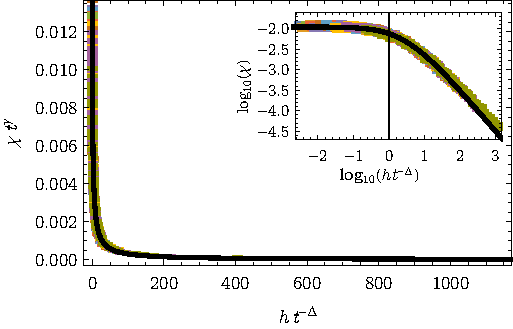
\includegraphics{figs/fig_sus-collapse}
  \caption{Fit of scaling form \eqref{eq:sus_scaling} to numeric data from a
  $L=1024$ square-lattice Ising model.
Different colored points show different values of $t$, which vary from
$0.01$, $0.02$, \dots, $0.1$. Solid black line shows fitted form, with
$C=0.0111\pm0.0023$ and $B=0.173\pm0.072$.}
  \label{fig:sus}
\end{figure}

\begin{figure}
  \input{figs/fig-mag}
  %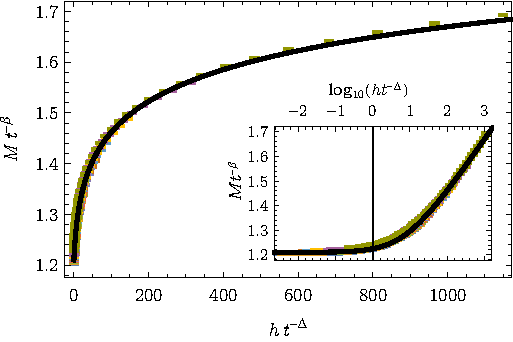
\includegraphics{figs/fig_mag-collapse}
  \caption{Fit of scaling form \eqref{eq:mag_scaling} to numeric data from a
$L=1024$ square-lattice Ising model. Different colored points show different
values of $t$, which vary from $0.01$, $0.02$, \dots, $0.1$. Solid black lines
shows fitted form, with $\mathcal M(0)=1.21039\pm0.00031$,
$D=0.09400\pm0.00035$, and $B=0.0861\pm0.0010$.}
  \label{fig:mag}
\end{figure}

The most accurate components of this analysis are its predictions for the
higher-order terms in the expansion
\[
  \mathcal F(X)=-\sum_{n=0}^\infty f_n(-X)^n
\]
\cite{brezin.1976.perturbation,bogomolny.1977.dispersion,lipatov.1977.divergence,parisi.1977.asymptotic}
which can be computed directly from the integral
\[
  f_n=\frac{(-1)^{n+1}}{n!}\pd{\mathcal F}X\bigg|_{X=0}
  =\frac{(-1)^{n+1}}{\pi}\int_{-\infty}^\infty\frac{\mathcal H(X)}{X^{n+1}}\;\dd X
\]
Applied to our ansatz \eqref{eq:im.scaling}, we find
\begin{align}
  f_n^{\text{\textsc{2d}}}
  &=\frac{AB^{n-1}\Gamma(n-1)}{\pi}
  &&
  n \geq 2
  \label{eq:fn.2d}
  \\
  f_n^{\text{\textsc{3d}}}
  &=\frac{AB^{n+\frac73}\Gamma(\frac n2+\frac76)}{2\pi}
  \\
  f_n^{\text{\textsc{4d}}}
  &=\frac{AB^{n+2}\Gamma(\frac n3+\frac23)}{3\pi}
\end{align}
The form of \eqref{eq:fn.2d} is identical to that found in
\cite{baker.1980.ising}, with our $f_n$ relating to their $a_n$ by
$a_{n-1}=2^nf_n$.
\[
  r_n=\frac{a_n}{a_{n-1}}=\frac{2f_{n+1}}{f_{n}}=2B\frac{\Gamma(n)}{\Gamma(n-1)}
\]

We have used results from the properties of the metastable Ising ferromagnet
and the analytic nature of the free energy to derive the universal scaling
functions for the free energy, and in \textsc{2d} the magnetization and
susceptibility, in the limit of small $t$ and $h$. Because of an essential
singularity in these functions at $h=0$---the abrupt transition line---their
form cannot be modified by analytic redefinition of control or thermodynamic
variables. These predictions match the results of simulations well. Having
demonstrated that the essential singularity in thermodynamic functions at the
abrupt singularity leads to observable effects we hope that these functional
forms will be used in conjunction with traditional perturbation methods to
better express the equation of state of the Ising model in the whole of its
parameter space.

\begin{acknowledgments}
  The authors would like to thank Tom Lubensky for a reason that Jim should
  really flesh out.
\end{acknowledgments}

\bibliography{essential-ising}

\end{document}

